% Chapter 5

\chapter{Produzione} % Main chapter title

\label{Chapter5} % Change X to a consecutive number; for referencing this chapter elsewhere, use \ref{ChapterX}

%----------------------------------------------------------------------------------------
%	SECTION 1
%----------------------------------------------------------------------------------------

\section{Modellazione}

Con modellazione digitale, o modellazione 3D, o semplicemente modellazione, per brevità, si intende la manipolazione di veritci in uno spazio tridimensionale per realizzare solidi più o meno complessi denominati modelli.
Questa è senz'altro la fare più artistica dell'intero processo di produzione, e una di quelle che più mi ha appassionato.

Una volta definiti i concept art, in gran parte realizzati da A. Uras, il primo passo della produzione è appunto quello di realizzare i modelli dei personaggi, dei prop e delle ambientazioni.
Per fare ciò, mi sono avvalso di diverse tecniche di modellazione 3D, che possono essere divise nelle seguenti 2 categorie:
\begin{itemize}
    \item Modellazione hard-surface \cite{hardSurf}.
    \item Scultura digitale\cite{3Dsculpt}.
\end{itemize}
La differenza fondamentale sta nel cosa si vuole realizzare. La prima è ottima per quasi tutto ciò che è realizzato dall'uomo (e.g. macchinari, edifici) ed è stata quindi stata usata nella realizzazione di ambientazioni e prop.
Consiste nel partire da una forma geometrica semplice, ad esempio un cubo o una sfera, ed aggiungere dettagli estrudendo sezioni o utilizzato operatori booleani in combinazione con altre forme geometriche. (Figura \ref{fig:box-model})
Il risultato è un modello dagli spigoli ben definiti, che comunque può avere superfici curve e smussate.
La caratteristica che lo distingue è la simmetria della struttura e la precisione della posizione dei dettagli. 

\begin{figure}
\centering
\begin{subfigure}{.5\textwidth}
  \centering
  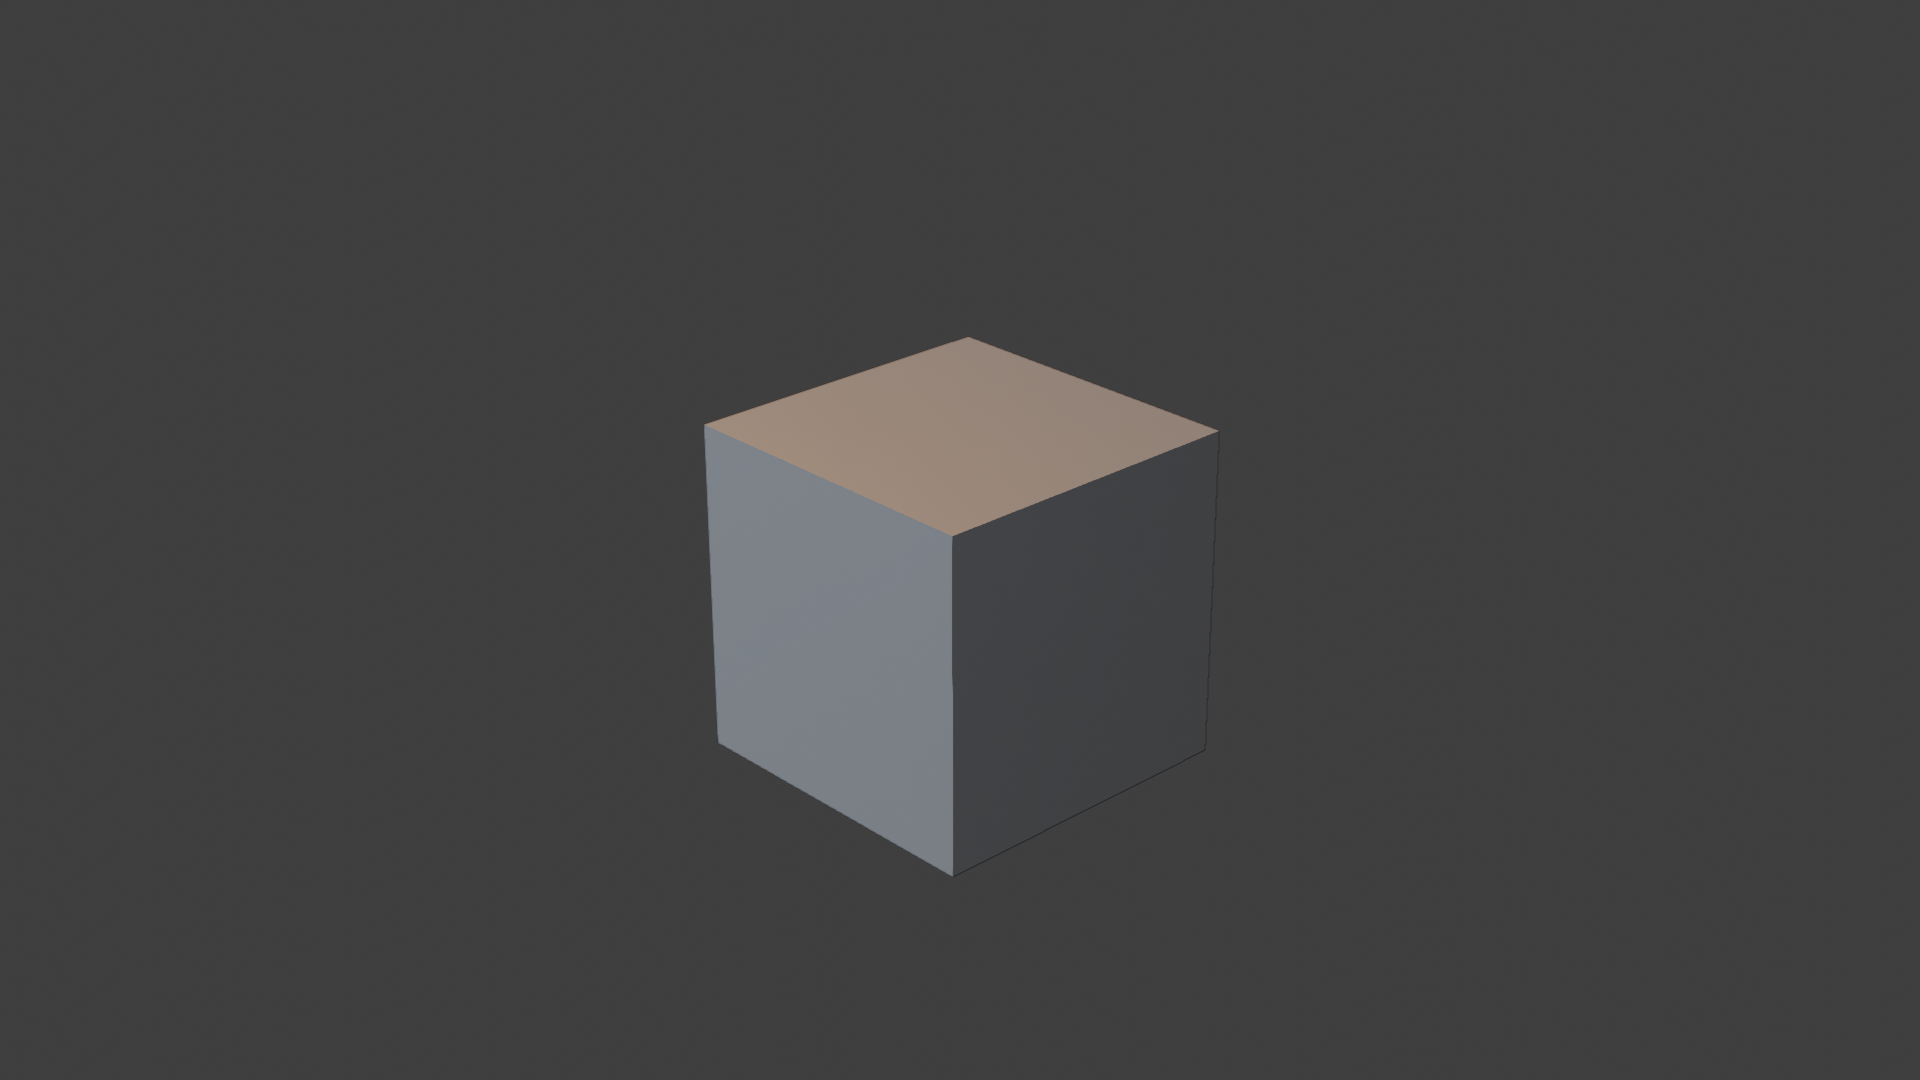
\includegraphics[width=.99\linewidth]{Figures/box1.png}
\end{subfigure}%
\begin{subfigure}{.5\textwidth}
  \centering
  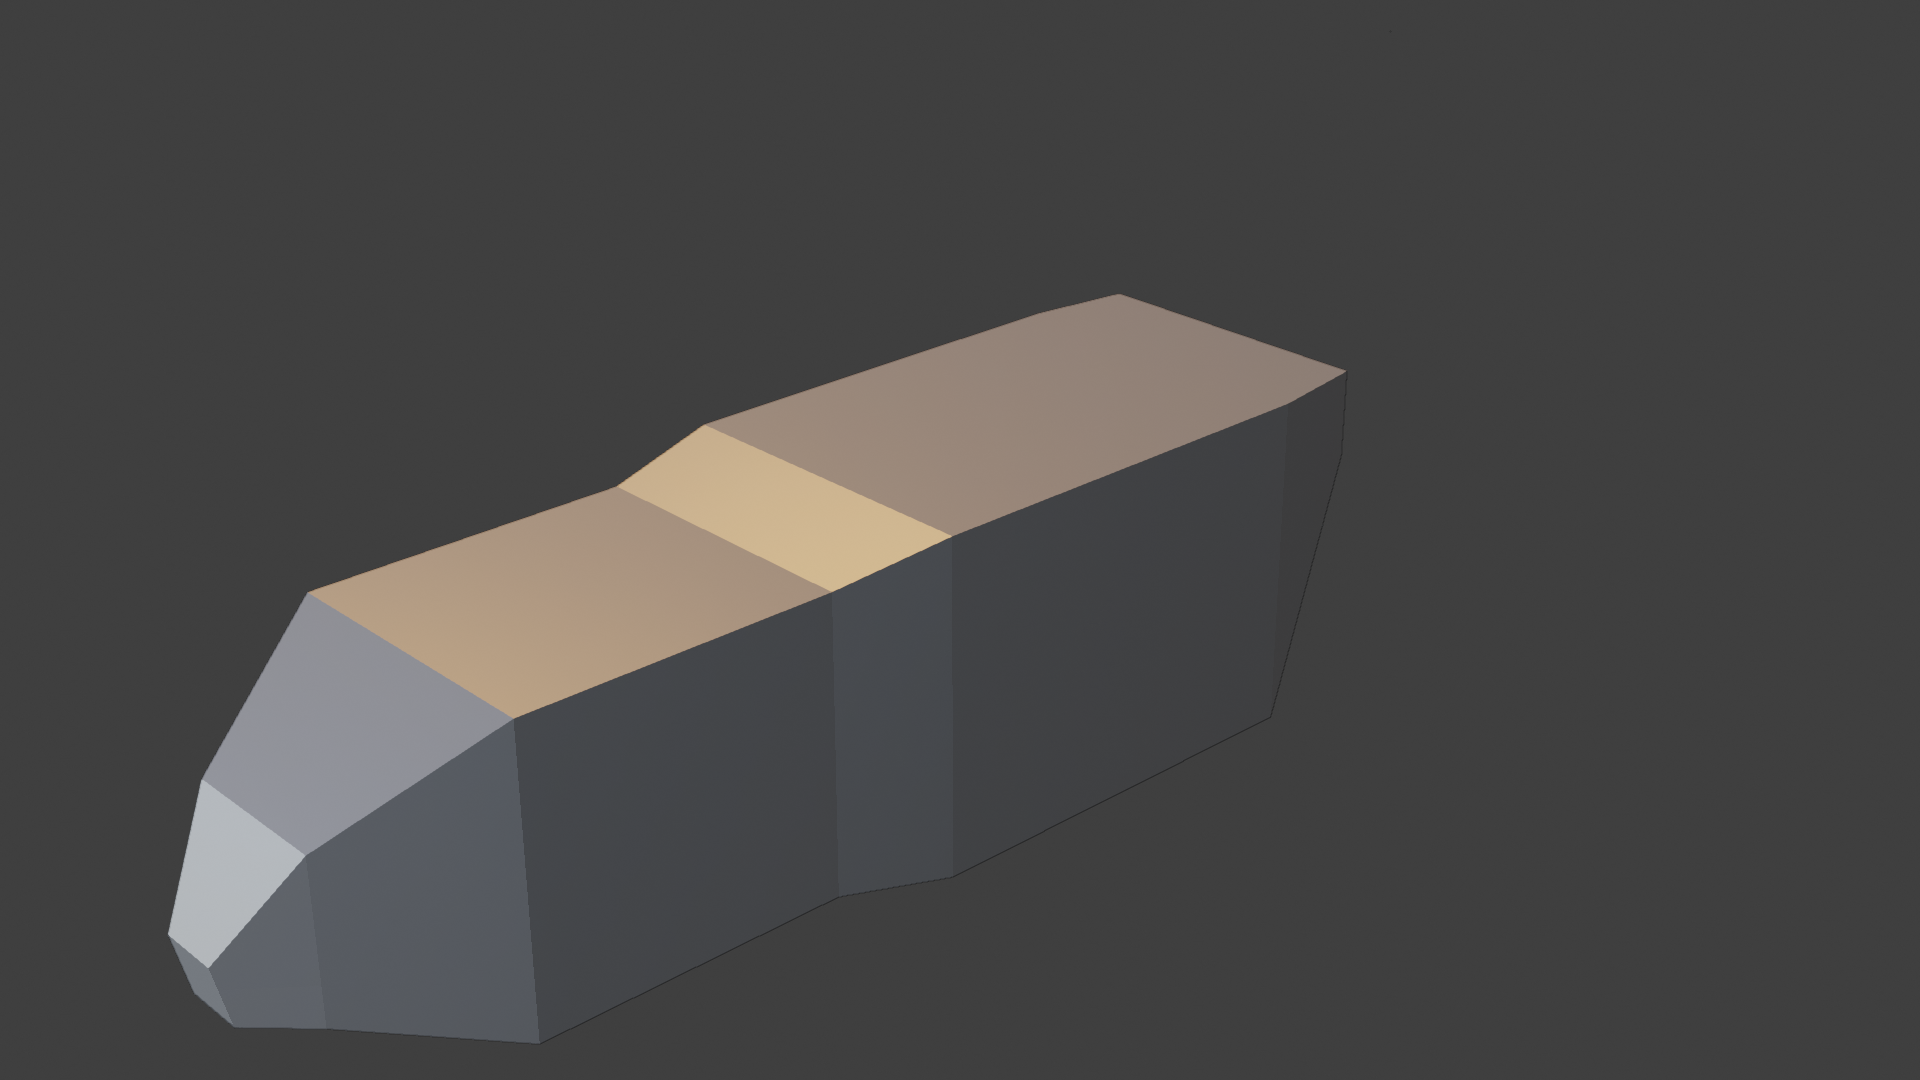
\includegraphics[width=.99\linewidth]{Figures/box2.png}
\end{subfigure}
\begin{subfigure}{.5\textwidth}
  \centering
  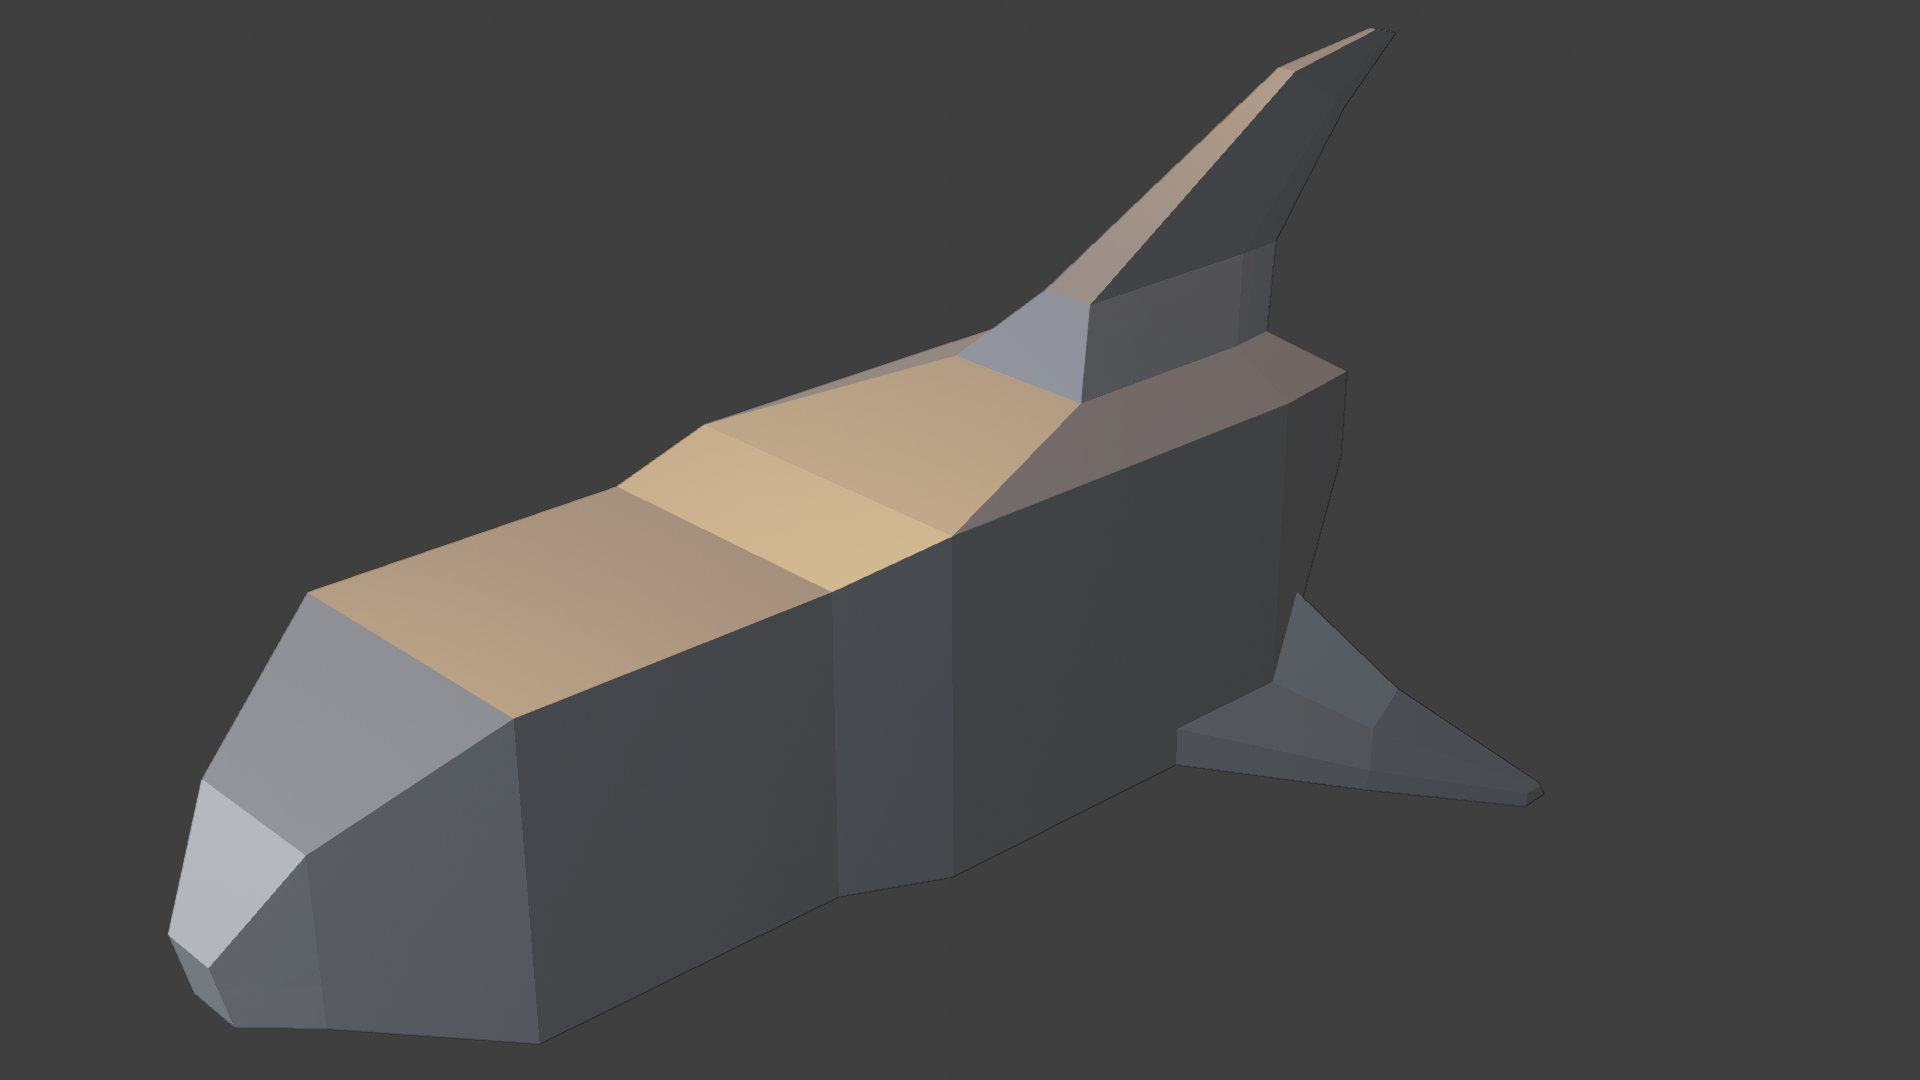
\includegraphics[width=.99\linewidth]{Figures/box3.png}
\end{subfigure}%
\begin{subfigure}{.5\textwidth}
  \centering
  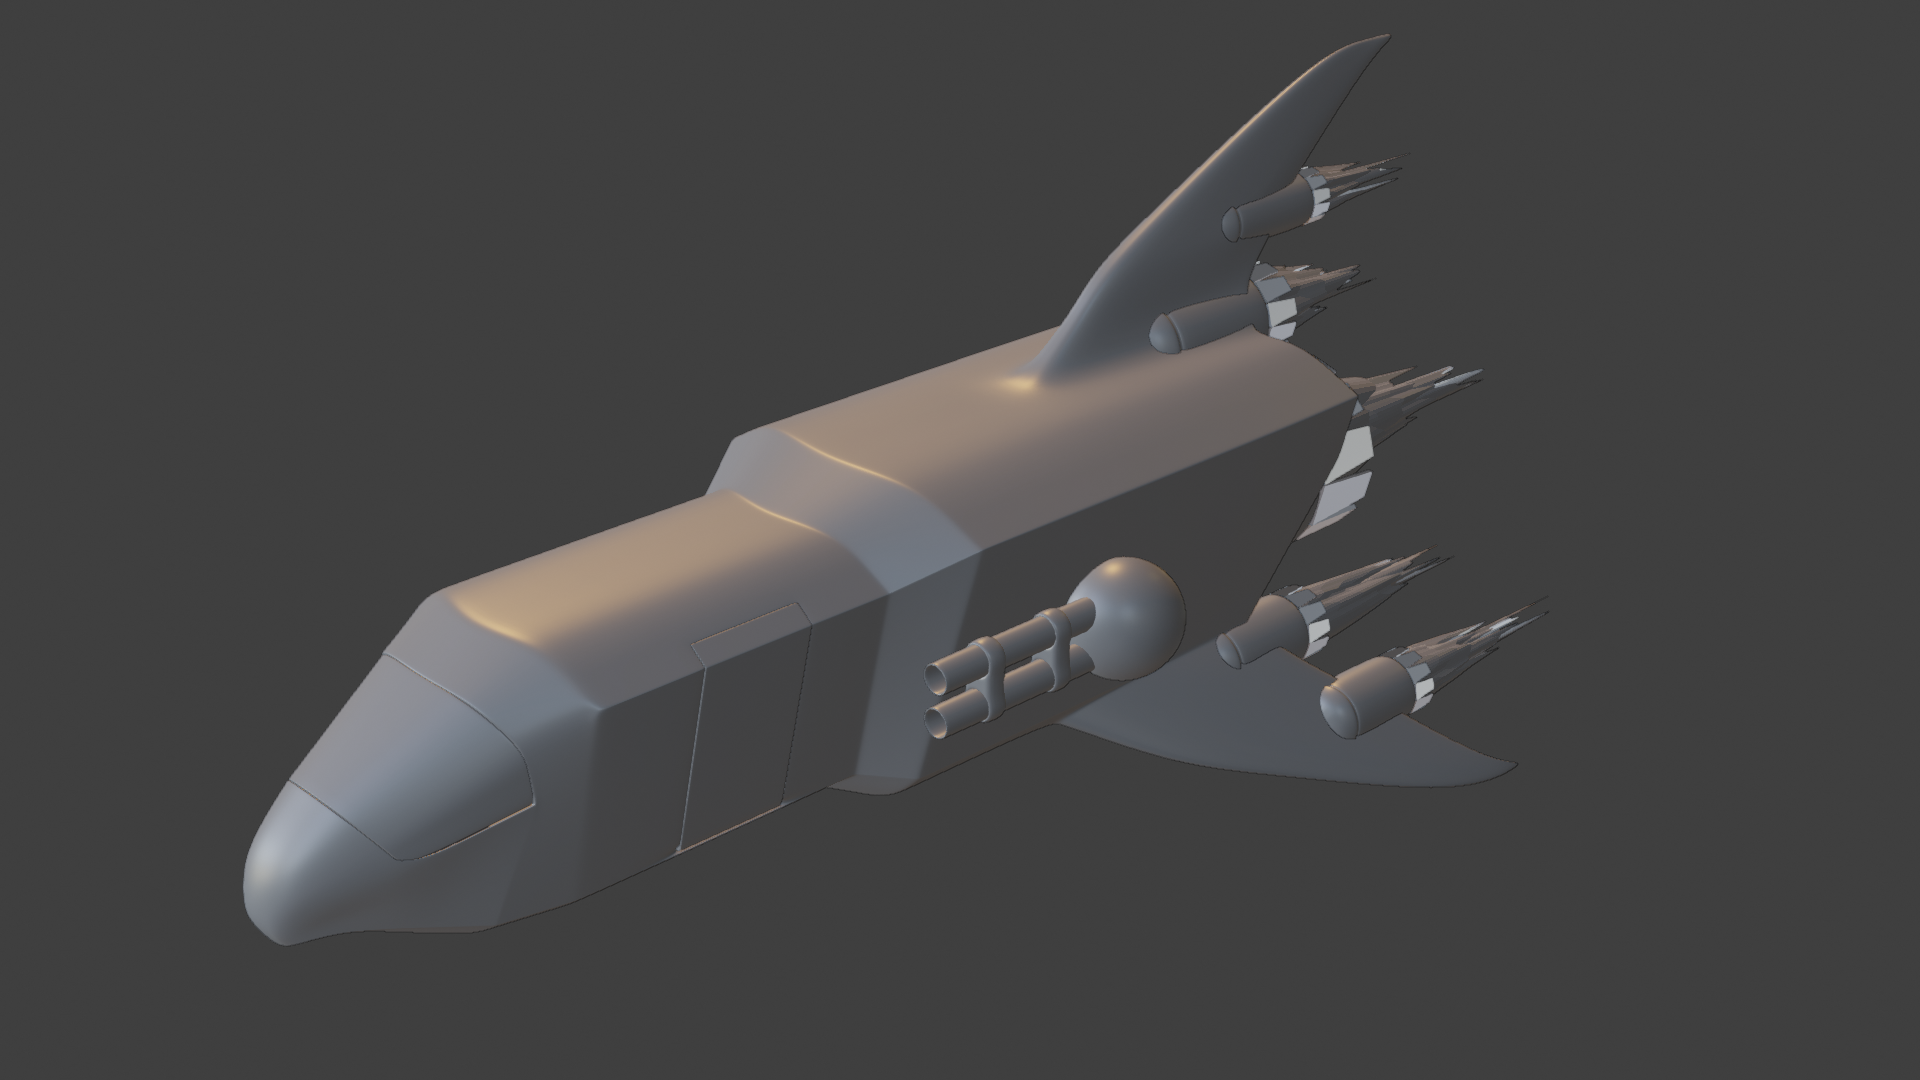
\includegraphics[width=.99\linewidth]{Figures/box4.png}
\end{subfigure}\\[2ex]
\decoRule
\caption[Modellazione hard-surface]{Esempio di modellazione hard-surface per modellare un'astronave.}
\label{fig:box-model}
\end{figure}

Al contrario, il secondo metodo viene utilizzato per ottenere modelli organici, in pratica tutto ciò che è presente in natura.
Questi modelli sono particolari, poiché andranno deformati per essere animati.
Un esempio lampante, in questo progetto, sono i personaggi.
Nonostante anche in questo caso la simmetria sia fondamentale (ogni personaggio ha 2 braccia e due gambe perfettamente simmetriche), vengono solitamente aggiunti dettagli per rompere la simmetria, siccome in natura nulla è perfettamente simmetrico.
Anche in questo caso si parte solitamente da delle forme geometriche semplici, tuttavia il processo di modellazione è completamente differente, tant'è che spesso si fa distinzione tra modellazione e scultura digitale (come se i due concetti si escludessero a vicenda).
Nella scultura digitale infatti non si usano mai operazioni come l'estrusione di una faccia, di fatto il concetto di faccia non viene neanche utilizzato.
La mesh viene vista come un oggetto compatto, i cui vertici possono essere manipolati attraverso strumenti che emulano le azioni di uno scultore.
Per questo motivo la scultura digitale è anche il metodo di modellazione preferito dagli artisti.
\newline

\begin{figure}
\centering
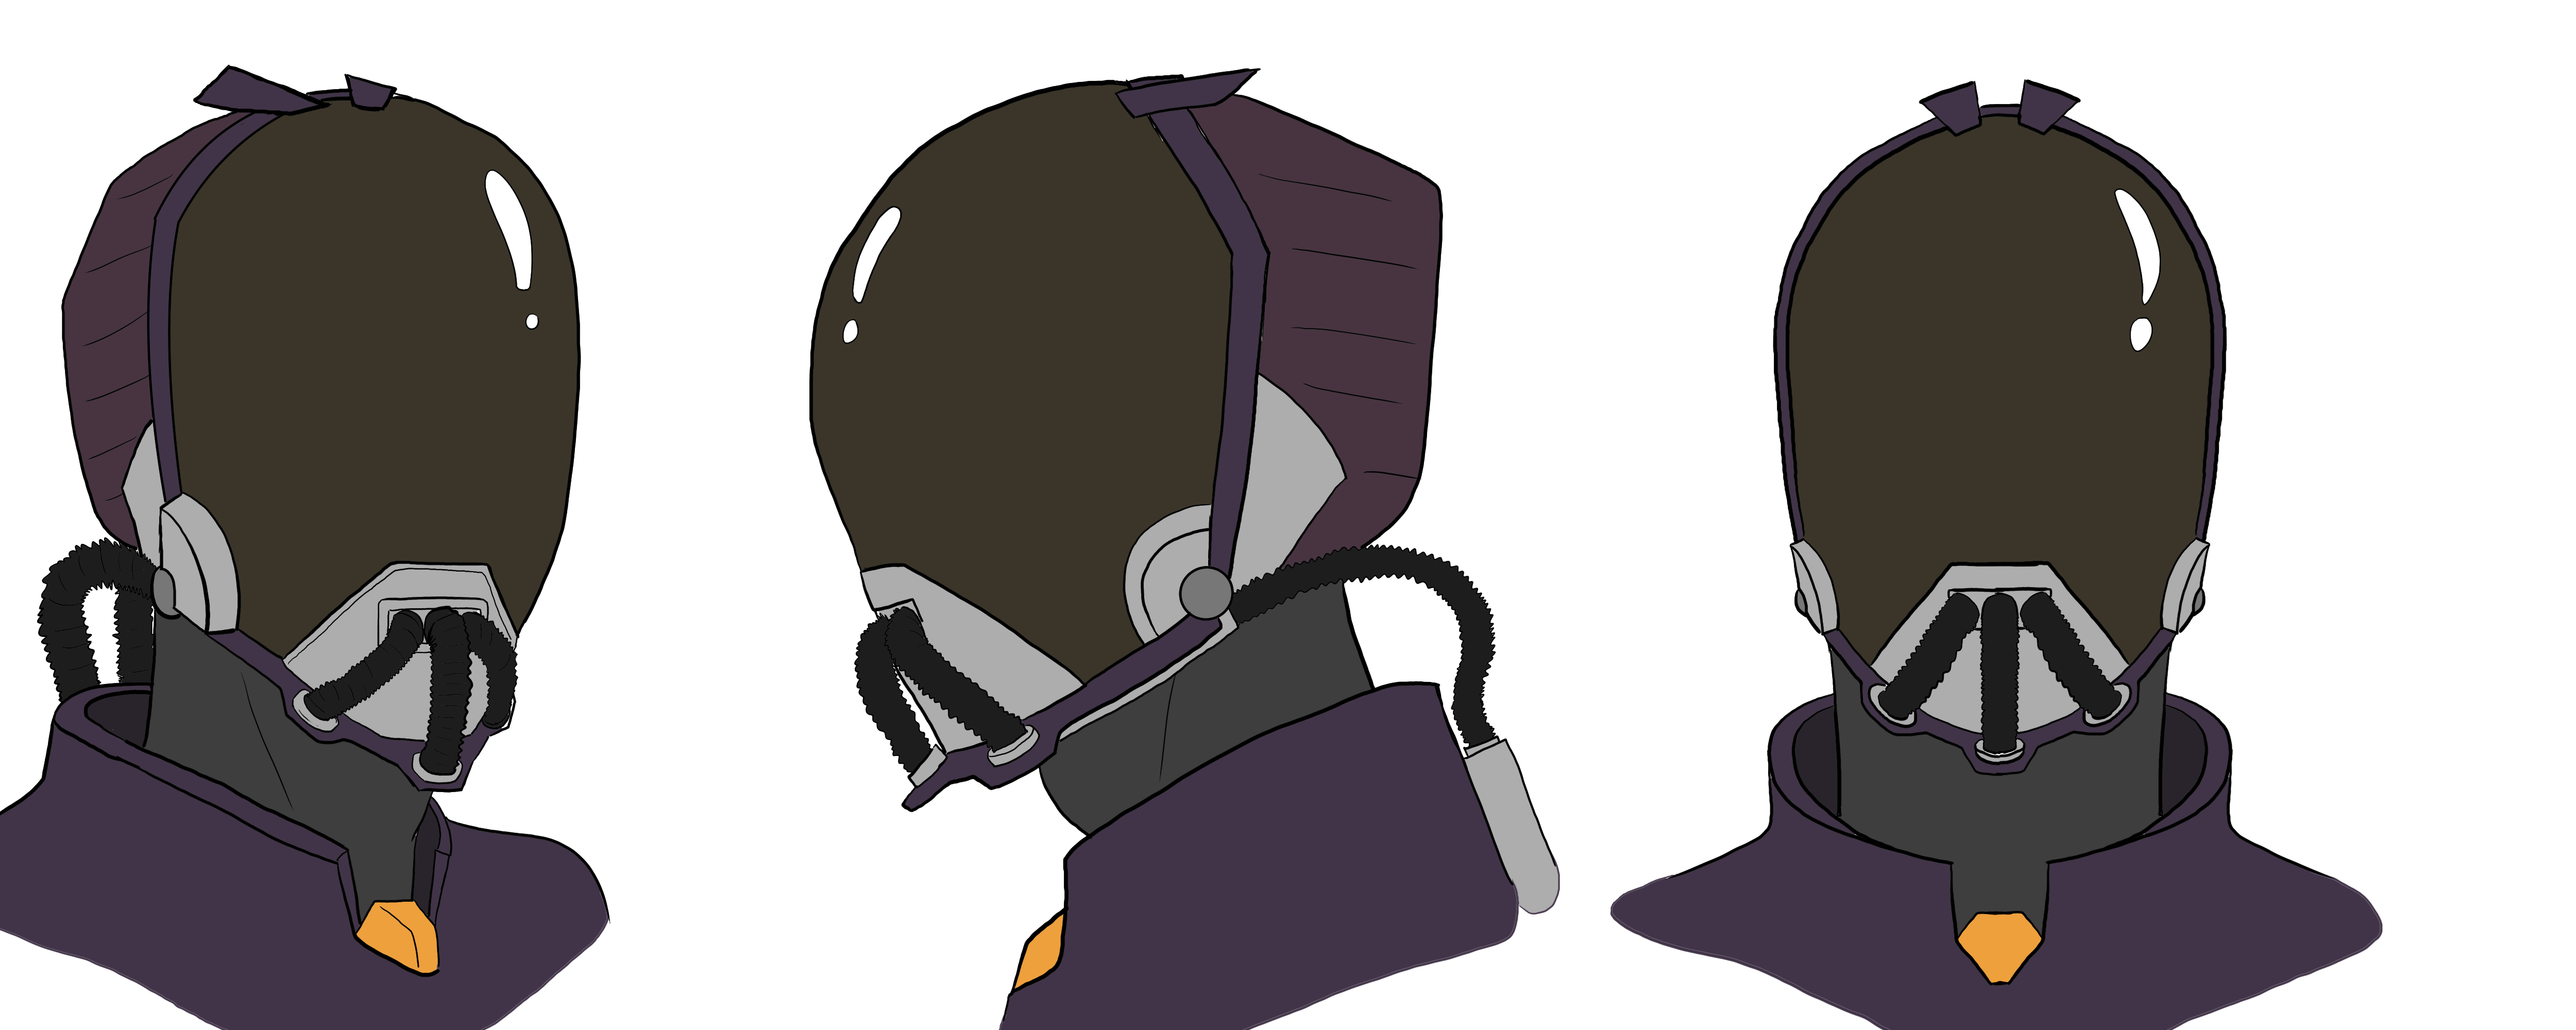
\includegraphics[width=.8\textwidth]{Figures/bandit-concept}
\decoRule
\caption[Concept art]{Concept art di uno dei porsonaggi}
\label{fig:concept}
\end{figure}
\begin{figure}
\centering
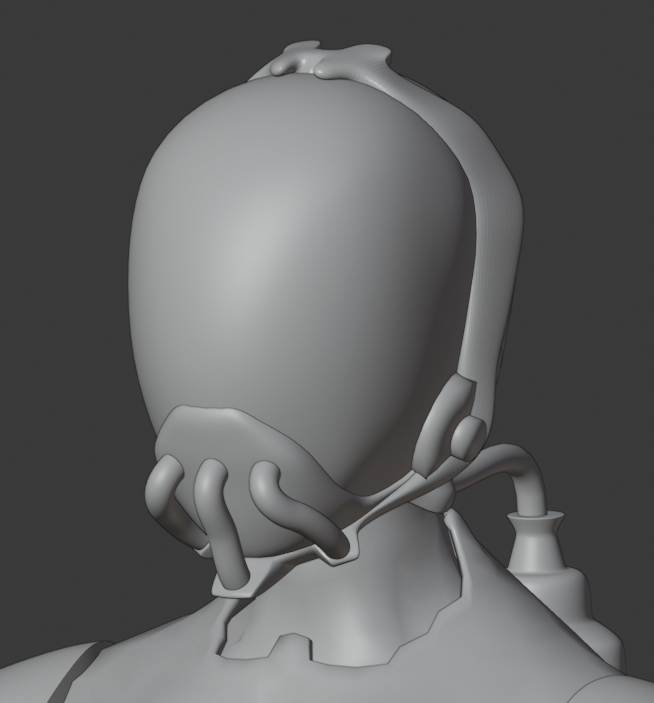
\includegraphics[width=.8\textwidth]{Figures/bandit-head}
\decoRule
\caption[Modello 3D]{Rappresentazione 3D del concept art mostrato in Figura \ref{fig:concept}}
\label{fig:model}
\end{figure}
Affinché un modello si possa definire ben fatto e ultimato, è necessario soddisfare i seguenti criteri.
In primo luogo, deve ben rappresentare in 3D quello che il concept si limitava a mostrare in 2D.
In Figura \ref{fig:concept} e \ref{fig:model} è possibile notare quanto il modello 3D si avvicini al concept originale.
Nonostante, in questo caso, il modello rappresenti molto bene il concept, è possibile notare come alcuni dettagli differiscano.
Questo è dovuto principalmente a due motivi: il primo è che, semplicemente, il concept art serve a dare un'idea di come deve apparire il personaggio, e non vincola quindi a mantenere gli stessi dettagli durante la fase di modellazione.
Il secondo è che in un disegno 2D la forzatura della prospettiva può nascondere dettagli a cui un modello 3D non può evadere.
Per tanto, sono spesso necessarie modifiche poiché non sarebbe possibile realizzare in 3D ciò che era rappresentato in 2D.

\begin{figure}
\centering
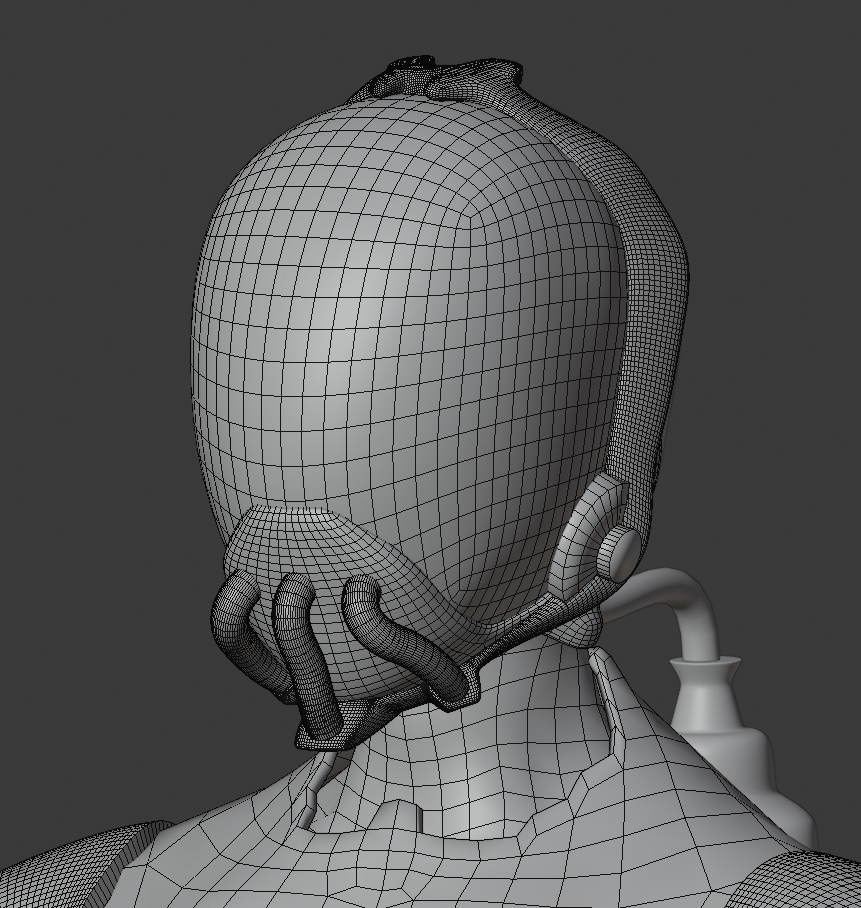
\includegraphics[width=.8\textwidth]{Figures/bandit-wire}
\decoRule
\caption[Topologia]{Modello 3D con topologia della mesh visibile}
\label{fig:wire}
\end{figure}
Il secondo criterio, non meno importante del primo, è la \emph{topologia} della mesh.
A dir la verità, questo aspetto non ha alcuna importanza nel caso di modelli statici, mirati allo scopo di essere rappresentati in un render fisso, o stampati in 3D.
Tuttavia, nel caso delle animazioni, questo è un aspetto fondamentale.
Infatti dal posizionamento dei vertici dipende la deformazione della mesh che, com'è già stato detto, è necessaria nelle animazioni dei modelli organici (e.g. personaggi).
Per avere una buona topologia, è fondamentale che le facce siano composte di quattro lati. Questo serve a definire dei percorsi, che attraversano la faccia da un lato a quello opposto e continuano nelle facce adiacenti.
Questi percorsi servono a far si che quando si aggiunge un maggiore livello di dettaglio, la mesh non venga deformata in maniera inaspettata.
Un altra caratteristica importante, per una buona topologia, è quella di avere al massimo quattro spigoli (o archi) che partano da ogni vertice.
Questo non è sempre possibile, tuttavia è necessario che vertici con più di cinque spigoli siano presenti nel minor numero possibile, e siano posizionati in punti strategici dove la mesh verrà difficilmente deformata.
Questo perché se vertice è adiacente a molti vertici, genera anche molti incroci di percorsi che sono da evitare per quanto detto prima.

Infine, un aspetto non poco importante nella definizione qualitativa di un modello, è il numero totale di vertici.
L'obiettivo è quello di avere il minor numero possibile di vertici per poter realizzare un certo livello di dettaglio.
Il motivo anche qui è duplice, seppure i due effetti sono strettamente correlati.
Innanzi tutto, un ridotto numero di vertici permette un \emph{frame-rate} più alto in fase di animazione.
In secondo luogo, in fase di rendering, ogni frame impiegerà meno tempo ad essere renderizzato.

Per mantenere un livello di dettaglio, discretamente alto, è stato fatto uso di una tecnica denominata \emph{baking}, che verrà approfondita nel paragrafo successivo.
Per ora mi limiterò a dire che per ogni modello è stato fatta prima una versione "\emph{low-poly}", ovvero a basso contenuto di poligoni (o vertici, analogamente).
Dopodiché i dettagli sono stati modellati su una copia di questo modello, dopo averne aumentato il numero di vertici suddividendo ogni faccia.
Avere due modelli separati, ci permette di utilizzare il primo nelle animazioni e, in un secondo momento, aggiungere i dettagli "cucinati".

Qui i vantaggi sono molteplici: è possibile iniziare ad animare un modello subito, parallelizzando la fase di animazione a quella di modellazione dei dettagli.
In più come già detto, si avrà un frame-rate più alto in fase di animazione, ed un rendering più veloce una volta ultimate le animazioni.

In Figura \ref{fig:boy} \ref{fig:cap} \ref{fig:lt} e \ref{fig:prop} sono riportati altri esempi di comparazione tra concept e modello 3D dei modelli da me realizzati. Tutti i concept, a parte quello del tenente, sono stati forniti da Alberto Uras. 
\begin{figure}
\centering
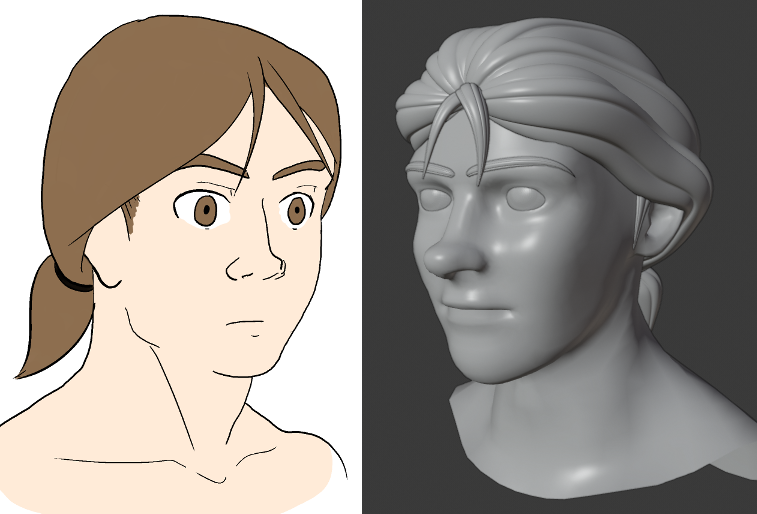
\includegraphics[width=.8\textwidth]{Figures/boy}
\decoRule
\caption[Ragazzo]{Modello 3D del volto del ragazzo a confronto con il relativo concept.}
\label{fig:boy}
\end{figure}
\begin{figure}
\centering
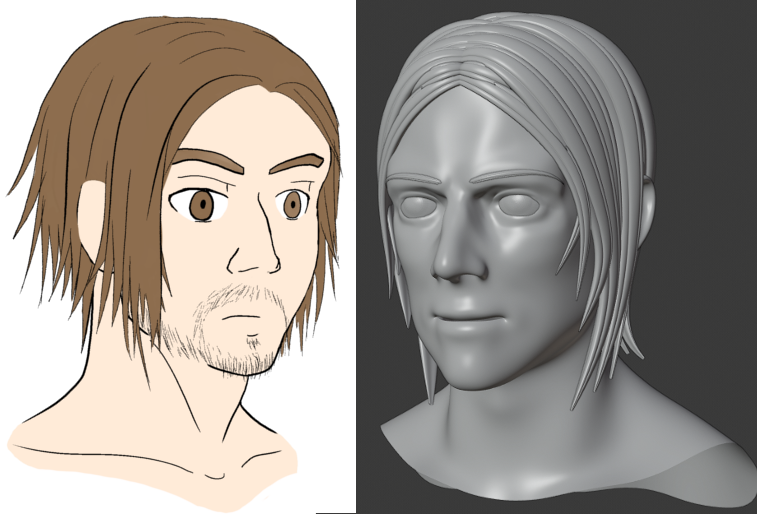
\includegraphics[width=.8\textwidth]{Figures/cap}
\decoRule
\caption[Capitano]{Modello 3D del volto del capt. Lawrence a confronto con il relativo concept.}
\label{fig:cap}
\end{figure}
\begin{figure}
\centering
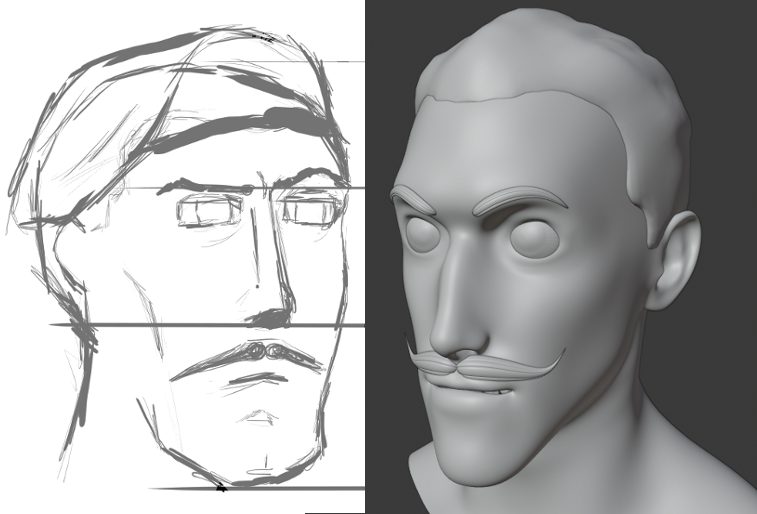
\includegraphics[width=.8\textwidth]{Figures/lt}
\decoRule
\caption[Tenente]{Modello 3D del volto del tenente a confronto con il relativo concept.}
\label{fig:lt}
\end{figure}
\begin{figure}
\centering
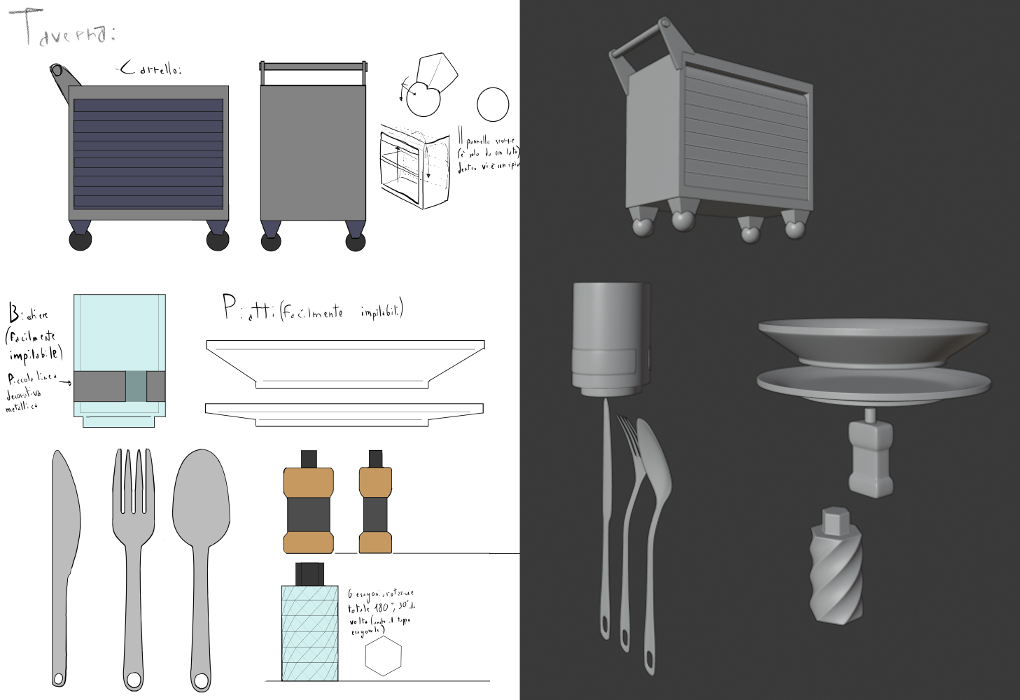
\includegraphics[width=.8\textwidth]{Figures/props}
\decoRule
\caption[Prop]{Alcuni modelli 3D dei prop a confronto con il relativo concept.}
\label{fig:prop}
\end{figure}

\section{Texturing}
Diverse tecniche:
painting manuale
geometria della mesh
generate proceduralmente

\section{Animazione e Rigging}

\begin{figure}
\centering
\begin{subfigure}{.33\textwidth}
  \centering
  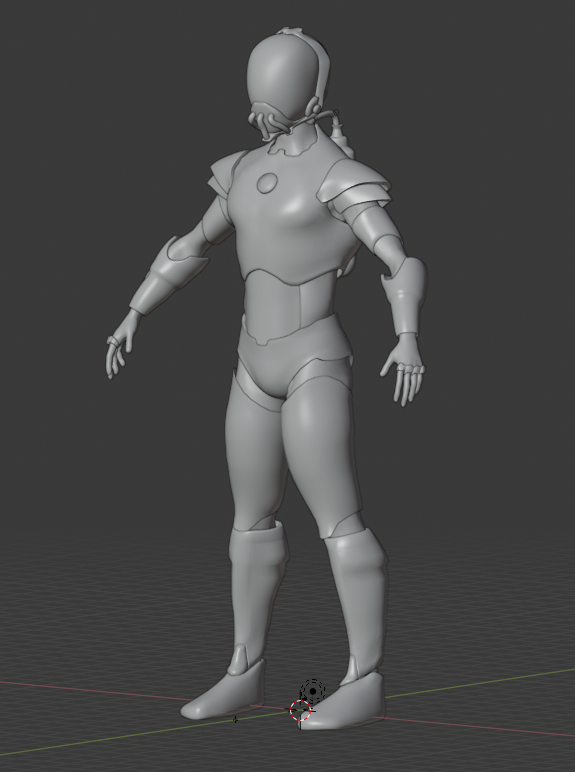
\includegraphics[width=\linewidth]{Figures/rig0}
  \caption{Modello senza controlli.\\}
  \vspace{13pt}
  \label{fig:rig0}
\end{subfigure}%
\begin{subfigure}{.33\textwidth}
  \centering
  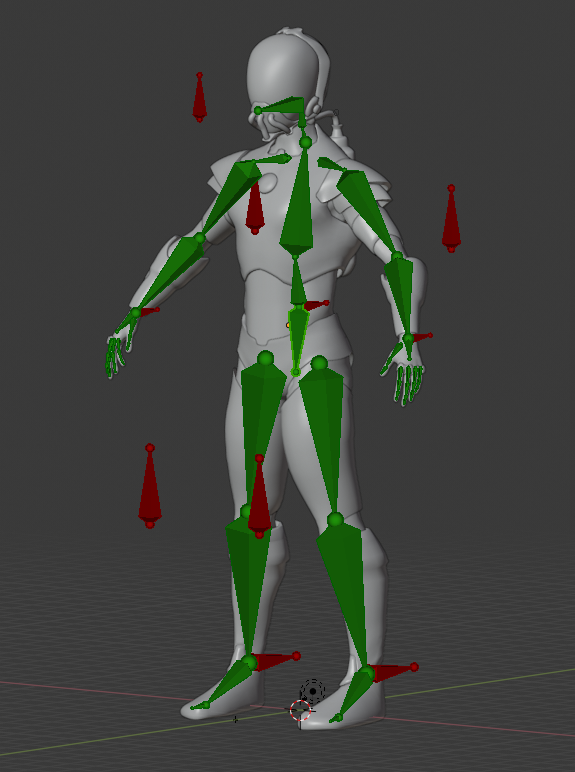
\includegraphics[width=\linewidth]{Figures/rig1}
  \caption{Armatura o meta-rig.}
  \bigskip
  \label{fig:rig1}
\end{subfigure}%
\begin{subfigure}{.33\textwidth}
  \centering
  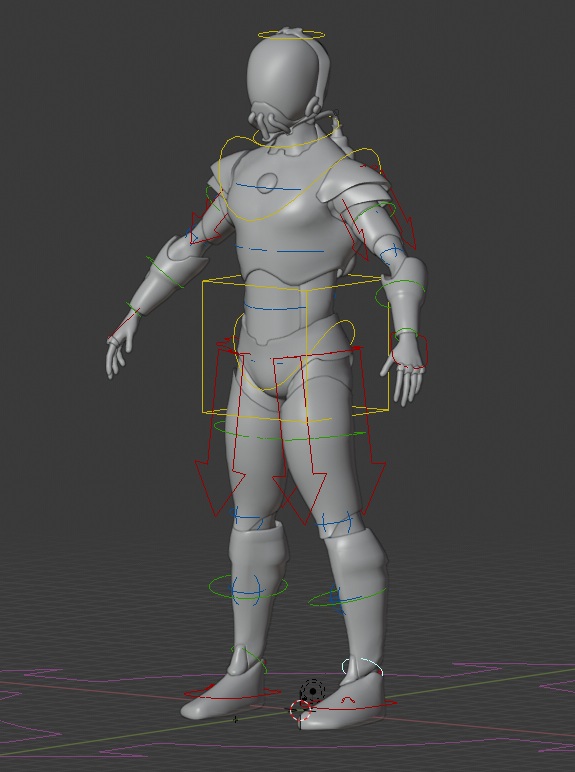
\includegraphics[width=\linewidth]{Figures/rig2}
  \caption{Rig avanzato con forme personalizzate.}
  \label{fig:rig2}
\end{subfigure}
\decoRule
\caption[Rig a confronto]{In figura è mostrato il modello di uno dei personaggi, con diversi tipi di controlli per l'animazione.}
\label{fig:rig}
\end{figure}

Rigging è un termine generale che si riferisce all'aggiunta di controlli ad un oggetto, tipicamente allo scopo di animarlo \parencite{blendDoc}.
Consiste nell'assegnare relazioni tra oggetti \parencite{BlendTut}.

menzionare rigify

Animazione straight ahead vs pose-to-pose (mixing between the 2)

dialoghi
menzionare Rhubarb

divisione dx/sx

\subsection{Cicli di animazione}
Il miglior modo per modulare un animazione, ovvero spezzarla in più azioni ripetibili, è quello di individuare le animazioni più frequenti (e.g. camminata, corsa) e definirle una sola volta.
Alcune animazioni, infatti, seguono dei pattern ben definiti.
Grazie alla loro uniformità è possibile renderle cicliche in maniera tale da non dover rifare la stessa animazione più volte.
\subsection{Shape keys}
Facial expression
uso di shape keys
ogni vertice è importante, inutile associare un osso per ogni gruppo di vertici: meglio avere diverse espressioni (set finito) e scegliere quale si vuole usare in base ad un valore reale (continuo)
\subsection{Drivers}
\subsection{Vincoli sulle azioni}
uno dei vantaggi dei vincoli sulle azioni è che è possibile animare le ossa vincolate direttamente, senza aggiungere un osso padre.

Solitamente utilizzate per controllare animazioni molto complesse, come la fuoriuscita del carrello di un aereo al momento dell'atterraggio, attraverso un solo controllo.

Reference
\begin{itemize}
    \item Dialog - The Animator's Survival Kit (p.304) 
    \item Facial animation - Algorithms\&Techniques (p.491)
    \item 3D production, animation - Finish you film (Production)
        \item create cycles for common actions - Finish you film (Production)
\end{itemize}
\section{Lighting}
\section{Rendering}

